\documentclass[14pt]{extarticle}
\usepackage[utf8]{inputenc}
\usepackage[T1]{fontenc}
\usepackage[spanish,es-lcroman]{babel}
\usepackage{amsmath}
\usepackage{amsthm}
\usepackage{physics}
\usepackage{tikz}
\usepackage{float}
\usepackage{calc}
\usepackage[autostyle,spanish=mexican]{csquotes}
\usepackage[per-mode=symbol]{siunitx}
\usepackage{gensymb}
\usepackage{multicol}
\usepackage{enumitem}
\usepackage{setspace}
\usepackage[left=2.00cm, right=2.00cm, top=2.00cm, 
     bottom=2.00cm]{geometry}
\usepackage{Estilos/ColoresLatex}
\usepackage{makecell}

% \usepackage[sfdefault]{roboto}  %% Option 'sfdefault' only if the base font of the document is to be sans serif
% \usepackage[T1]{fontenc}

\usepackage{scalerel}[2016-12-29]
\def\stretchint#1{\vcenter{\hbox{\stretchto[440]{\displaystyle\int}{#1}}}}
\def\scaleint#1{\vcenter{\hbox{\scaleto[3ex]{\displaystyle\int}{#1}}}}
\def\bs{\mkern-12mu}

\newcommand{\textocolor}[2]{\textbf{\textcolor{#1}{#2}}}
\sisetup{per-mode=symbol}
\decimalpoint
\sisetup{bracket-numbers = false}
\newlength{\depthofsumsign}
\setlength{\depthofsumsign}{\depthof{$\sum$}}
\newcommand{\nsum}[1][1.4]{% only for \displaystyle
    \mathop{%
        \raisebox
            {-#1\depthofsumsign+1\depthofsumsign}
            {\scalebox
                {#1}
                {$\displaystyle\sum$}%
            }
    }
}

\title{\vspace*{-2cm} Lentes gruesas y sistemas de varias lentes}
\date{ }

\begin{document}
\maketitle

\section{Distancias focales efectivas y planos principales.}

Es posible demostrar fácilmente, con el uso de las ecuaciones II.14 y II.24, que la amplificación dada por una lente delgada cuya distancia focal $f$ es mucho más corta que la distancia $l_{1}$ está dada aproximadamente por:
\begin{align}
m = \dfrac{f}{l_{1}}
\label{eq:ecuacion_III_01}
\end{align}
Por otro lado, usando el teorema de Lagrange visto anteriomente, la amplificación
de un sistema óptico formado por una o varias lentes, gruesas o delgadas, está dada por:
\begin{align}
m = \dfrac{u}{u^{\prime}} = - \dfrac{y_{1}}{l_{1} \, u^{\prime}}
\label{eq:ecuacion_III_02}
\end{align}
La ecuación (\ref{eq:ecuacion_III_01}) es válida hasta ahora únicamente para lentes delgadas, mientras que la ecuación (\ref{eq:ecuacion_III_02}) tiene validez general. Aquí vemos la inconveniencia de que la distancia focal efectiva $f$ de un sistema de lentes se defina como:
\begin{align}
f = - \dfrac{y_{1}}{u^{\prime}}
\label{eq:ecuacion_III_03}
\end{align}
a fin de que la ecuación (\ref{eq:ecuacion_III_01}) sea también válida para sistemas de varias lentes, gruesas o delgadas, con ejes ópticos coincidentes. A un sistema de lentes con eje óptico común se le llama en general \textit{sistema óptico centrado}. Desde luego, la expresión (\ref{eq:ecuacion_III_01}) tiene la misma restricción original de que $l_{1}$ sea mucho mayor que $f$, tal cual se ve en la figura (\ref{fig:figura_III_01a}).
\begin{figure}[H]
    \centering
    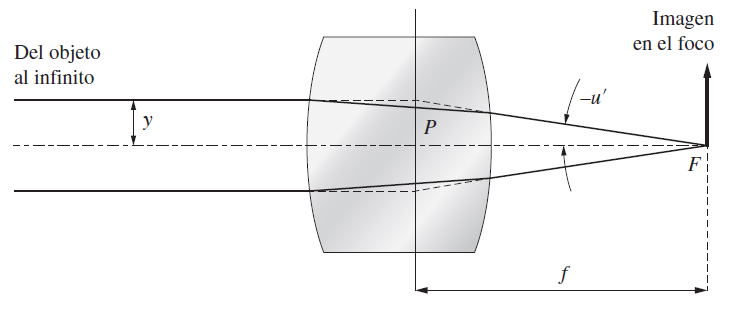
\includegraphics[scale=0.7]{Imagenes/Lentes_Gruesas_01.png}
    \caption{Amplificación lateral con un sistema de lentes.}
    \label{fig:figura_III_01}
\end{figure}
Para ser más rigurosos, consideraremos que el objeto está casi en el infinito y que por tanto los rayos llegan a la lente en haces paralelos entre sí. Como es natural, la amplificación $m$ es casi cero pero no exactamente, porque $l_{1}$ podrá ser muy grande pero nunca infinita.

Examinando la figura (\ref{fig:figura_III_01}) vemos que la distancia focal efectiva $f$ representa la distancia del foco a un plano imaginario definido por las intersecciones de prolongaciones de los rayos incidentes y los rayos refractados finales. Este plano imaginario recibe el nombre de \textit{plano principal} del sistema.

En general existen dos diferentes planos principales en un sistema de lentes,
dependiendo de si la luz llega al sistema de un objeto a la izquierda o a la derecha de él, como se muestra en la figura (\ref{fig:figura_III_02}).
\begin{figure}[H]
    \centering
    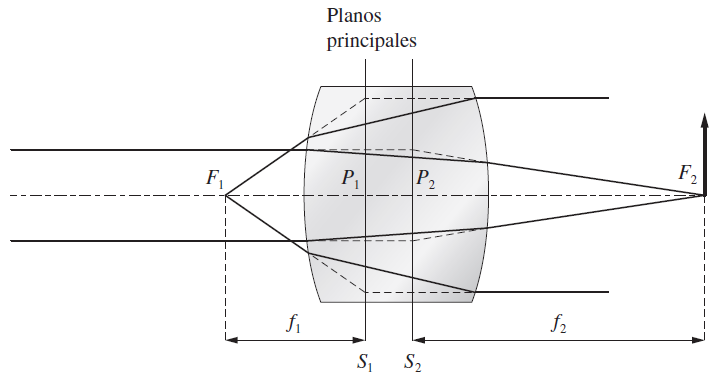
\includegraphics[scale=0.7]{Imagenes/Lentes_Gruesas_02.png}
    \caption{Amplificación lateral con un sistema de lentes.}
    \label{fig:figura_III_02}
\end{figure}
En esta figura se han definido de manera gráfica:
\begin{enumerate}[label=\alph*)]
\item los planos principales $S_{1}$ y $S_{2}$.
\item los puntos principales $P_{1}$ y $P_{2}$.
\item las distancias focales efectivas $f_{1}$ y $f_{2}$.
\end{enumerate}
Es interesante notar que un sistema puede ser aparentemente convergente y, sin
embargo, tener distancia focal efectiva negativa. También podría ser en apariencia
divergente y tener distancia focal efectiva positiva. Esto sucede cuando el rayo cruza el eje óptico un número par de veces antes de salir del sistema de lentes.

\subsection{Potencia de un sistema óptico.}

La distancia focal efectiva de un sistema óptico compuesto por varias superficies esféricas centradas se puede encontrar con ayuda de la fórmula de Gauss (ecuación
I.34). Si usamos las relaciones $u = y/l$ y $u^{\prime} = - y/l^{\prime}$, en esta relación encontraremos:
\begin{align}
n^{\prime} \ , u^{\prime} = - n \, u = - y \left( \dfrac{n^{\prime} - n}{r} \right)
\label{eq:ecuacion_III_04}
\end{align}
Sumando ambos lados para un sistema de $k$ superficies se obtiene:
\begin{align}
n_{k}^{\prime} \ , u_{k}^{\prime} = - n \, u = - \nsum_{i=1}^{k} y_{i} \left( \dfrac{n_{i}^{\prime} - n_{i}}{r_{i}} \right)
\label{eq:ecuacion_III_05}
\end{align}
usando la definición de la distancia focal efectiva $f$ dada por la ecuación (\ref{eq:ecuacion_III_03}) y haciendo $u_{1} = 0$, obtenemos:
\begin{align}
\dfrac{1}{f} = \nsum_{i=1}^{k} \dfrac{y_{i}}{y_{1}} \left( \dfrac{n_{i}^{\prime} - n_{i}}{n_{k}^{\prime} \, r_{i}} \right)
\label{eq:ecuacion_III_06}
\end{align}
Si se particulariza ahora para un sistema de $k$ lentes delgadas en aire $(n_{k}^{\prime} = 1)$ cuyas distancias focales individuales son $f_{i}$.

\section{Amplificación lateral y puntos conjugados.}

Algunas propiedades importantes relativas a la formación de imágenes con un sistema
de lentes se pueden encontrar con el solo uso de la definición de distancias focal
efectiva y el teorema de Lagrange. Para ello consideraremos la figura (\ref{fig:figura_III_03}).
\begin{figure}[H]
    \centering
    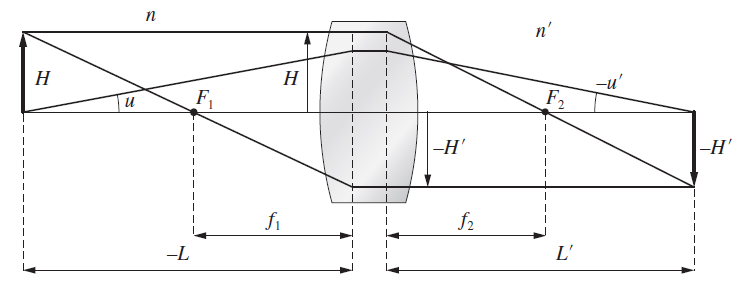
\includegraphics[scale=0.7]{Imagenes/Lentes_Gruesas_03.png}
    \caption{Formación de imágenes con un sistema de lentes.}
    \label{fig:figura_III_03}
\end{figure}
La amplificación lateral se puede encontrar utilizando el teorema de Lagrange
como sigue:
\begin{align}
m = \dfrac{H^{\prime}}{H} = \dfrac{n \, u}{n^{\prime} \, u^{\prime}}
\label{eq:ecuacion_III_08}
\end{align}
Si se usa ahora una aproximación para rayos paraxiales podemos escribir:
\begin{align}
\dfrac{u}{u^{\prime}} =  \dfrac{L^{\prime}}{L}
\label{eq:ecuacion_III_09}
\end{align}
y al sustituir esta relación en la ecuación (\ref{eq:ecuacion_III_08}), se obtiene:
\begin{align}
m = \dfrac{H^{\prime}}{H} = \dfrac{n \, L^{\prime}}{n^{\prime} \, L}
\label{eq:ecuacion_III_10}
\end{align}
La ecuación (\ref{eq:ecuacion_III_10}) es equivalente a la ecuación II.24 para lentes delgadas.

De la figura (\ref{fig:figura_III_03}), que se construyó usando solamente las definiciones de planos principales y distancias focales efectivas, podemos obtener:
\begin{align}
\dfrac{- H}{H} = \dfrac{L^{\prime} - f_{2}}{f_{2}}
\label{eq:ecuacion_III_11}
\end{align}
y
\begin{align}
\dfrac{- H}{H} = \dfrac{f_{1}}{-L - f_{1}}
\label{eq:ecuacion_III_12}
\end{align}
Ahora, igualando estas dos expresiones:
\begin{align}
L \, L\ {\prime} = f_{2} \, L - f_{1} \, L^{\prime}
\label{eq:ecuacion_III_13}
\end{align}
de donde vemos que:
\begin{align}
L^{\prime} - f_{2} = - \dfrac{f_{1} \, L^{\prime}}{L}
\label{eq:ecuacion_III_14}
\end{align}
expresión que sustituimos en la ecuación (\ref{eq:ecuacion_III_11}), así obtenemos:
\begin{align}
\dfrac{H^{\prime}}{H} = \dfrac{f_{1} \, L}{f_{2} \, L}
\label{eq:ecuacion_III_15}
\end{align}
Igualando ahora las ecuaciones (\ref{eq:ecuacion_III_10}) y (\ref{eq:ecuacion_III_15}) obtenemos la expresión equivalente a la II.11 para lentes delgadas:
\begin{align}
n \, f_{2} = n^{\prime} \, f_{1}
\label{eq:ecuacion_III_16}
\end{align}
Como ya se revisó anteriormente, casi siempre $n = n^{\prime}$ y por lo tanto $f_{1} = f_{2}$.

Tres excepciones posibles son:

\begin{enumerate}[label=\roman*)]
\item una cámara submarina, donde el objeto está en agua y la imagen en aire.
\item un microscopio con objetivo de inmersión, donde el objeto está en aceite y la
imagen en aire.
\item el ojo humano, donde el objeto está en aire y la imagen en el humor vítreo.
\end{enumerate}
De las ecuaciones (\ref{eq:ecuacion_III_13}) y (\ref{eq:ecuacion_III_16}) podemos obtener la expresión análoga a la II.13 para conseguir la posición de la imagen dada la posición del objeto y viceversa:
\begin{align}
\dfrac{1}{f_{2}} = \dfrac{1}{L^{\prime}} - \dfrac{n}{n^{\prime} \, L}
\label{eq:ecuacion_III_17}
\end{align}
Si $n = n^{\prime}$, esta expresión se reduce a la análoga a la ecuación II.14 para lentes delgadas:
\begin{align}
\dfrac{1}{f} = \dfrac{1}{L^{\prime}} - \dfrac{1}{L}
\label{eq:ecuacion_III_18}
\end{align}

\section{Puntos nodales.}

Los puntos nodales de un sistema óptico centrado son dos puntos $N_{1}$ y $N_{2}$ sobre el eje óptico, con la siguiente propiedad: \enquote{Si un rayo entra al sistema óptico dirigiéndose de forma aparente al punto nodal $N_{1}$, saldrá del sistema paralelamente al rayo incidente y con su prolongación pasando por el punto nodal $N_{2}$}. Con el auxilio de la figura (\ref{fig:figura_III_04}) encontraremos la posición de los puntos nodales sobre el eje óptico.
\begin{figure}[H]
    \centering
    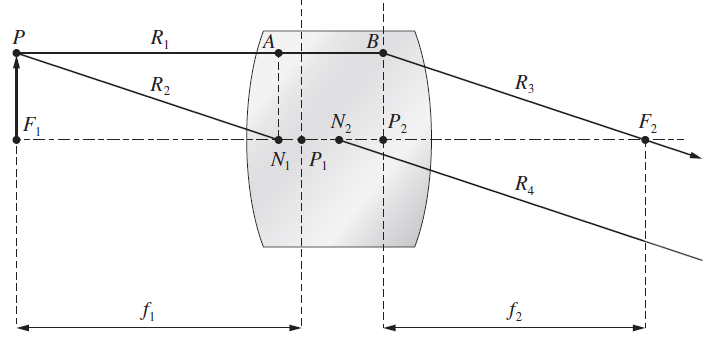
\includegraphics[scale=0.7]{Imagenes/Lentes_Gruesas_04.png}
    \caption{Puntos nodales de un sistema de lentes.}
    \label{fig:figura_III_04}
\end{figure}
Consideremos un punto $P$ sobre el plano focal que contiene al foco $F_{1}$. Si los
rayos $R_{1}$ y $R_{2}$ parten de $P$, saldrán del sistema óptico como dos rayos $R_{3}$ y $R_{4}$ paralelos entre sí. Escojamos el rayo $l_{2}$ de tal forma que apunte al punto nodal $N_{1}$ y entonces, por definición de punto nodal, el rayo $l_{4}$ saldrá con su prolongación pasando por el punto nodal $N_{2}$. Como los rayos $l_{3}$ y $l_{4}$ son paralelos entre sí, el rayo $l_{3}$ es también paralelo a $l_{2}$. Por lo tanto, se puede ver que los triángulos $PAN_{1}$ y $F_{2} P_{2} B$ son idénticos. De aquí que las distancias $\overline{F_{1} N_{1}}$ y $\overline{P_{2} F_{2}}$ sean iguales y, por consiguiente, podamos escribir:
\begin{align}
\overline{F_{1} N_{1}} = f_{2}
\label{eq:ecuacion_III_19}
\end{align}
La distancia del punto nodal $N_{1}$ al punto principal $P_{1}$, según podemos observar en la figura (\ref{fig:figura_III_04}), está entonces dada por:
\begin{align}
\overline{N_{1} P_{1}} = f_{1} - \overline{F_{1} N_{1}} = f_{1} - f_{2}
\label{eq:ecuacion_III_20}
\end{align}
Usando ahora la ecuación (\ref{eq:ecuacion_III_16}), esta distancia se puede escribir:
\begin{align}
\overline{N_{1} P_{1}} = \left( 1 - \dfrac{n^{\prime}}{n} \right) f_{1}
\label{eq:ecuacion_III_21}
\end{align}
Por simetría, la distancia del punto nodal $N_{2}$ al punto principal $P_{2}$ está dada por:
\begin{align}
\overline{N_{2} P_{2}} = \left( 1 - \dfrac{n^{\prime}}{n} \right) f_{2}
\label{eq:ecuacion_III_22}
\end{align}
Estas dos expresiones son las análogas de la ecuación II.26 para una lente delgada.
Si el primero y el último medios tienen el mismo índice de refracción $(n = n^{\prime})$, los dos puntos nodales coinciden con los puntos correspondientes. Tanto a los puntos principales como a los puntos nodales se les da con frecuencia el nombre genérico de \textit{puntos cardinales}.

\section{Lentes gruesas.}

Uno de los sistemas ópticos centrados no delgados más sencillos es el formado por una lente gruesa simple. Toda la teoría desarrollada en este capítulo para los sistemas ópticos centrados se aplica de manera directa a las lentes gruesas. Para completar el estudio de una lente de este tipo sólo falta encontrar las expresiones para las distancias focales efectiva y posterior.

\subsection{Distancia focal efectiva.}

La distancia focal efectiva de una lente gruesa se puede encontrar con la fórmula de Gauss para una superficie esférica refractora y con la ayuda de la figura (\ref{fig:figura_III_06}).
\begin{figure}[H]
    \centering
    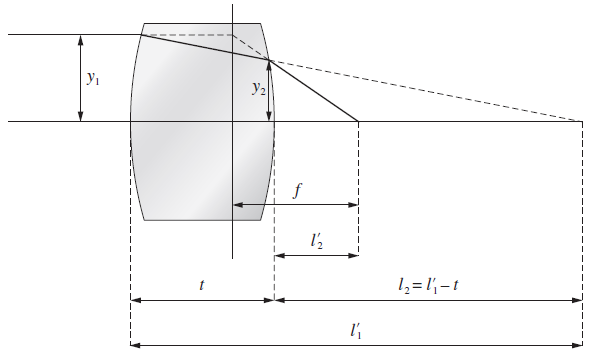
\includegraphics[scale=0.7]{Imagenes/Lentes_Gruesas_05.png}
    \caption{Refracción de un rayo meridional paraxial en una lente gruesa.}
    \label{fig:figura_III_06}
\end{figure}
De la figura se puede ver que:
\begin{align}
\dfrac{y_{1}}{f} = \dfrac{y_{2}}{l_{2}^{\prime}}
\label{eq:ecuacion_III_23}
\end{align}
y que:
\begin{align}
\dfrac{y_{1}}{l_{1}^{\prime}} = \dfrac{y_{2}}{l_{1}^{\prime} - t}
\label{eq:ecuacion_III_24}
\end{align}
donde $t$ es el grueso central de la lente. Eliminando $y_{1}$ y $y_{2}$ de estas dos ecuaciones encontramos:
\begin{align}
\dfrac{1}{f} = \dfrac{l_{1}^{\prime} - t}{l_{1}^{\prime} \, l_{2}^{\prime}}
\label{eq:ecuacion_III_25}
\end{align}
Si sustituimos $l_{2} = l_{1}^{\prime} - t$ en la fórmula de Gauss, para la segunda superficie podemos obtener:
\begin{align}
\dfrac{1}{l_{2}^{\prime}} = \dfrac{n}{l_{1}^{\prime} - t} - \dfrac{n - 1}{r_{2}}
\label{eq:ecuacion_III_26}
\end{align}
y si ahora sustituimos $l_{1} = \infty \quad 1/l_{1} \rightarrow \infty$ en la fórmula de Gauss para la primera superficie:
\begin{align}
\dfrac{n}{l_{1}^{\prime}} = \dfrac{n - 1}{r_{1}}
\label{eq:ecuacion_III_27}
\end{align}
en estas dos expresiones se han hecho las sustituciones $n_{2} = n_{1}^{\prime}$ y $n_{1} = n_{2}^{\prime} = 1$.

Si sustituimos ahora el valor de $l_{2}^{\prime}$ de la ecuación (\ref{eq:ecuacion_III_26}) en la ecuación (\ref{eq:ecuacion_III_25}) obtenemos:
\begin{align}
\dfrac{1}{f} = \dfrac{n}{l_{1}^{\prime}} - \dfrac{l_{1}^{\prime} - t}{l_{1}^{\prime \left( \dfrac{n - 1}{r_{2}} \right)}}
\label{eq:ecuacion_III_28}
\end{align}
Sustituyendo ahora el valor de $l_{1}^{\prime}$ de la ecuación (\ref{eq:ecuacion_III_27}) en la ecuación (\ref{eq:ecuacion_III_28}) encontramos finalmente:
\begin{align}
\dfrac{1}{f} = (n - 1) \left( \dfrac{1}{r_{1}} - \dfrac{1}{r_{2}} \right) + \dfrac{t (n - 1)^{2}}{n \, r_{1} \, r_{2}}
\label{eq:ecuacion_III_29}
\end{align}
Como es lógico, cuando $t = 0$ esta expresión se reduce a la equivalente para lentes delgadas. Si el grueso de la lente es pequeño comparado con $r_{1}$ y $r_{2}$, la contribución del segundo término es pequeña comparada con la del primero.

\subsection{Distancia focal posterior.}

Por definición, la distancia focal posterior es la distancia $l_{2}^{\prime}$ que se puede obtener sustituyendo el valor de $l_{1}^{\prime}$ de la ecuación (\ref{eq:ecuacion_III_27}) en la ecuación (\ref{eq:ecuacion_III_26}):
\begin{align}
\dfrac{1}{l_{2}^{\prime}} = (n - 1) \left[ \dfrac{1}{r_{1} \left( 1 - \dfrac{(n - 1) t}{r_{1} \, n} \right)} - \dfrac{1}{r_{2}} \right]
\label{eq:ecuacion_III_30}
\end{align}
Cuando $t$ tiende a cero, la distancia $l_{2}^{\prime}$ tiende al valor de la distancia focal de una lente delgada. La figura (\ref{fig:figura_III_07a}) - (\ref{fig:figura_III_07b}) muestra las posiciones aproximadas de los planos principales para una lente gruesa, según su forma.
\begin{figure}[H]
    \centering
    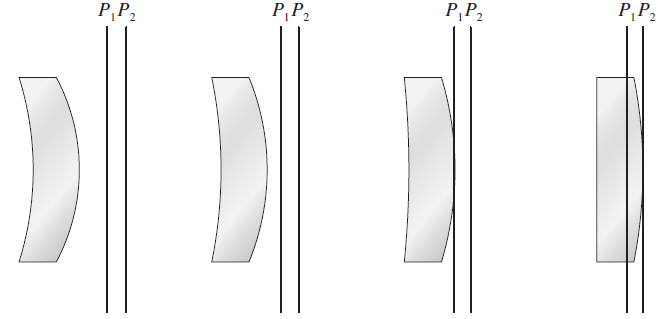
\includegraphics[scale=0.7]{Imagenes/Lentes_Gruesas_06a.png}
    \caption{Ubicación de los planos principales en una lente convergente. La distancia focal efectiva es la misma en todas las lentes, únicamente cambia su forma.}
    \label{fig:figura_III_07a}
\end{figure}
\begin{figure}[H]
    \centering
    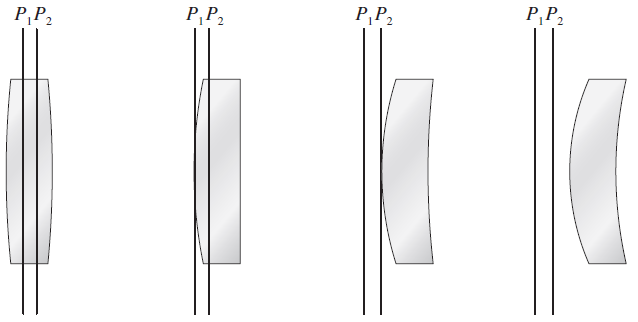
\includegraphics[scale=0.7]{Imagenes/Lentes_Gruesas_06b.png}
    \caption{Ubicación de los planos principales en una lente convergente. La distancia focal efectiva es la misma en todas las lentes, únicamente cambia su forma.}
    \label{fig:figura_III_07b}
\end{figure}

\section{Sistema de dos lentes delgadas.}

Otro ejemplo muy simple de sistema óptico centrado grueso es el sistema formado por dos lentes delgadas separadas por una distancia d mayor que cero. Al igual que para una lente gruesa encontraremos ahora las distancias focales efectiva y posterior para un sistema de dos lentes delgadas.

\subsection{Distancia focal efectiva.}

Esta distancia se calculará con ayuda de la figura (\ref{fig:figura_III_08}):
\begin{figure}[H]
    \centering
    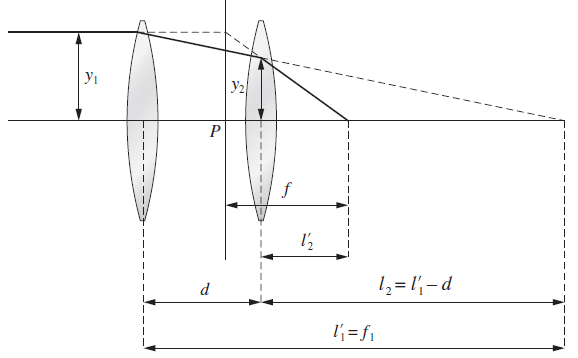
\includegraphics[scale=0.7]{Imagenes/Lentes_Sistema_01.png}
    \caption{Refracción de un rayo meridional paraxial en un sistema de dos lentes delgadas.}
    \label{fig:figura_III_08}
\end{figure}
donde podemos ver que:
\begin{align}
\dfrac{y_{1}}{f} = \dfrac{y_{2}}{l_{2}^{\prime}}
\label{eq:ecuacion_III_31}
\end{align}
Si eliminamos de las dos últimas ecuaciones $y_{1}$ y $y_{2}$:
\begin{align}
\dfrac{1}{f} = \dfrac{l_{1}^{\prime} - d}{l_{1} \, l_{2}}
\label{eq:ecuacion_III_33}
\end{align}
pero como la luz llega colimada al sistema, tenemos que $l_{1}^{\prime}$, y por lo tanto:
\begin{align}
\dfrac{1}{f} = \dfrac{f_{1} - d}{f_{1} \, l_{2}^{\prime}}
\label{eq:ecuacion_III_34}
\end{align}
Por otro lado, aplicando la ecuación:
\begin{align*}
\dfrac{1}{f} = \dfrac{1}{l_{2}^{\prime}} - \dfrac{1}{l_{1}}
\end{align*}
a la segunda lente:
\begin{align}
\dfrac{1}{f_{2}} = \dfrac{1}{l_{2}^{\prime}} - \dfrac{1}{f_{1} - d}
\label{eq:ecuacion_III_35}
\end{align}
y de aquí podemos despejar $l_{2}^{\prime}$ para sustituirla en la ecuación (\ref{eq:ecuacion_III_34}), así obtenemos:
\begin{align}
\dfrac{1}{f} = \dfrac{1}{f_{1}} + \dfrac{1}{f_{2}} - \dfrac{d}{f_{1} \ f_{2}}
\label{eq:ecuacion_III_36}
\end{align}
Si las dos lentes están en contacto una con otra, esta expresión se reduce a:
\begin{align}
\dfrac{1}{f} = \dfrac{1}{f_{1}} + \dfrac{1}{f_{2}}
\label{eq:ecuacion_III_37}
\end{align}

\subsection{Distancia focal posterior.}

Por definición, la distancia focal posterior es la distancia $l_{2}^{\prime}$, que se puede obtener directamente de la ecuación (\ref{eq:ecuacion_III_35}) como:
\begin{align}
\dfrac{1}{l_{2}^{\prime}} = \dfrac{1}{f_{1} - d} + \dfrac{1}{f_{2}}
\label{eq:ecuacion_III_38}
\end{align}
Como es natural, la ecuación (\ref{eq:ecuacion_III_38}) se reduce a la ecuación (\ref{eq:ecuacion_III_37}) con $l_{2}^{\prime} = f$ cuando $d = 0$.

\end{document}




